\documentclass[runningheads]{llncs}
\usepackage{algorithm,algorithmic,amsfonts,bm,hyperref,booktabs,tikz,pgf,pgfplots,amsmath,soul,subcaption,url,graphicx,amsmath,booktabs,booktabs,nicefrac,bm,colortbl,tikz,pgfplots,enumerate,xargs}
\usetikzlibrary{arrows,automata,circuits}
\captionsetup{compatibility=false}
\usetikzlibrary{arrows,plotmarks,decorations.markings,trees,shapes}
\tikzstyle{nodo}=[ellipse,draw=black!100,fill=black!30,line width=.7pt,minimum width=1.2cm,minimum height=.7cm]
\tikzstyle{Qnodo}=[ellipse,draw=black!100,fill=black!10,line width=.7pt,minimum width=1.2cm,minimum height=.7cm]
\tikzstyle{arco}=[draw=black!80,line width=.7pt, postaction={decorate}, decoration={markings,mark=at position 1.0 with {\arrow[ draw=black!80,line width=.7pt]{>}}}]
\tikzstyle{decision} = [rectangle, draw, fill=black!100,text=white, text width=4.5em, text badly centered, node distance=3cm, minimum height=3em]
\tikzstyle{block} = [rectangle, draw, fill=blue!20, text width=5em, text centered, rounded corners, minimum height=3em]
\tikzstyle{line} = [draw, -latex']
\tikzstyle{cloud} = [draw, ellipse,fill=red!20, node distance=3cm, minimum height=2em]
\def\mystrut{\vphantom{hg}}
\pgfplotsset{legend image with text/.style={
legend image code/.code={%
\node[anchor=center] at (0.3cm,0cm) {#1};}},}
\pgfplotsset{compat=1.13}
\begin{document}
\title{A New Score for Adaptive Tests\\in Bayesian and Credal Networks}
\author{Alessandro Antonucci \and
Francesca Mangili \and\\
Claudio Bonesana \and
Giorgia Adorni}
%%\thanks{Supported by organization x.}}
%\titlerunning{A New ScoreAbbreviated paper title}
\authorrunning{Antonucci et al.}
\institute{Istituto Dalle Molle di Studi sull'Intelligenza Artificiale, Lugano, Switzerland\\
\email{\{alessandro,francesca,claudio.bonesana,giorgia.adorni\}@idsia.ch}}
\maketitle
\begin{abstract}
A test is \emph{adaptive} when its sequence and number of questions is dynamically tuned on the basis of the estimated skills of the taker. Graphical models, such as Bayesian networks, are used for adaptive tests as they allow to model the uncertainty about the questions and the skills in an explainable fashion, especially when coping with multiple skills. A better elicitation of the uncertainty in the question/skills relations can be achieved by interval probabilities. This turns the model into a \emph{credal} network, thus making the inferential complexity of the queries required to select questions more demanding. This is especially the case for the information theoretic quantities used as \emph{scores} to drive the adaptive mechanism. We present an alternative family of scores, based on the mode of the posterior probabilities and hence easier to explain. This makes considerably simpler the evaluation in the credal case, without significantly affecting the quality of the adaptive process. Numerical tests on synthetic and real-world data are used to support this claim.
%12 pages
\keywords{Computer adaptive tests \and Information theory \and Credal networks \and Bayesian networks}
\end{abstract}
\section{Introduction}\label{sec:intro}
A test or an exam can be naturally intended as a measurement process, with the questions acting as sensors measuring the skills of the test taker in a particular discipline. Such measurement is typically imperfect with the skills acting as latent variables whose actual values cannot be revealed in a perfectly reliable way. The role of the questions, whose answers are regarded instead as manifest variables, is to reduce the uncertainty about the latent skills. Following this perspective, probabilistic modelling is an obvious framework to describe tests. Consider for instance the example in Figure \ref{fig:minicat}, where a small Bayesian network is used to describe the probability of the test taker having understood how to multiply numbers. In such a framework making the test \emph{adaptive}, i.e., picking a next question on the basis of the current knowledge level of the test taker is also very natural. The expected information gain for the available questions might be naturally used to select the question leading to the more informative results about the skill level of the test taker. This might take place before the answer to the question on the basis of the expectations about the possible answers.

A critical point when coping with such approaches is to provide a realistic assessment for the probabilistic parameters associated with the modelling of the relations between the questions and the skills. Having to provide sharp numerical values for these probabilities might be difficult. As the skill is typically a latent quantity, complete data are not available for a statistical learning of the parameters and the elicitation should therefore demanded to experts (e.g., a teacher). Yet, it might be not obvious to express such a domain knowledge by single numbers and a more robust elicitation, such as a probability interval, might add realism and robustness to the modelling process \cite{hajek2012rationality}. With such generalized assessments of the parameters a Bayesian network simply becomes a \emph{credal} network \cite{antonucci2010d}. Yet, the counterpart of such increased realism is the higher computational complexity characterizing the inference in credal networks \cite{maua14jair}. This is especially the case when coping with information theoretic measures such a information gain, whose computation might lead to complex non-linear optimization tasks \cite{mangili2017b}. The goal of this paper is to investigate the potential of alternatives to the information-theoretic scores driving the question selection in adaptive tests based on directed graphical models, no matter whether these are Bayesian or credal networks. In particular, we consider a family of scores based on the (expected) mode of the posterior distributions over the skills. We show that, when coping with credal networks, the computation of these scores can be reduced to the simpler optimization tasks involving multi-linear optimizations for which powerful approximation schemes are already available \cite{antonucci2013a}. Moreover, we show that these scores benefit of better explainability properties, thus allowing for a more transparent process in the question selection.

\begin{figure}[htp!]
\centering
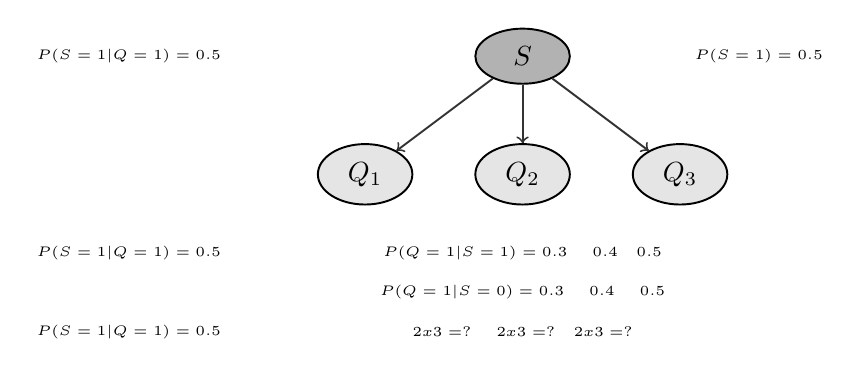
\begin{tikzpicture}[scale=1]
\node[] ()  at (-5,0.5) {\tiny $P(S=1|Q=1)=0.5$};
\node[] ()  at (-5,-2) {\tiny $P(S=1|Q=1)=0.5$};
\node[] ()  at (-5,-3) {\tiny $P(S=1|Q=1)=0.5$};
\node[] ()  at (3,0.5) {\tiny $P(S=1)=0.5$};
\node[] ()  at (0,-3) {\tiny $2x3=?$ \quad $2x3=?$\quad  $2x3=?$};
\node[] ()  at (0,-2) {\tiny $P(Q=1|S=1)=0.3$ \quad $0.4$\quad  $0.5$};
\node[] ()  at (0,-2.5) {\tiny $P(Q=1|S=0)=0.3$ \quad  $0.4$ \quad  $0.5$};
\node[nodo] (s)  at (0,0.5) {$S$};
\node[Qnodo] (q1)  at (-2.,-1) {$Q_1$};
\node[Qnodo] (q2)  at (0,-1) {$Q_2$};
\node[Qnodo] (q3)  at (2,-1) {$Q_3$};
\draw[arco] (s) -- (q1);
\draw[arco] (s) -- (q2);
\draw[arco] (s) -- (q3);
\end{tikzpicture}
\caption{Ad adaptive testing scheme to evaluate the multiplication (Boolean) skill $S$ by three (Boolean) questions. Probabilities are assessed by the Bayesian network on the right}
    \label{fig:minicat}
\end{figure}
*** espandere figura ***
\newpage 
The paper is organized as follows. A critical discussion about the existing work in this area is in Section \ref{sec:work}. The necessary background material is reviewed in Section \ref{sec:background}. The adaptive testing concepts are introduced in Section \ref{sec:cat} and specialized to graphical models in \ref{sec:bncat}. The technical part of the paper is in Section \ref{sec:mode}, where the new scores are discussed and specialized to the credal case, while the experiments are in Section \ref{sec:exp}. Conclusions and outlooks are in Section \ref{sec:conc}.

\section{Related Work}\label{sec:work}
Modelling a test as a process involving latent variables is a classical approach since the proposal of the classical \emph{item response theory}, that has been widely used even to implement adaptive sequences \cite{xxx}. Despite its success related to the ease of implementation and inference, IRT might be inadequate when coping with multiple latent skill, especially when these are dependent. For such cases, interpretable graphical models such as Bayesian networks have been resulted more effective [x]. The development of (computer) adaptive tests is a classical topic for AI \cite{xx}. Apart from graphical models, adaptive algorithms have been proposed within a genetic optimization framework. The idea of using Bayesian network in grading environment is not new. xxx. As already noticed in the previous section, the latent nature of the student skills might hinder the direct statistical learning of the parameters of such models. This naturally led some authors to consider missing data modelling. In particular the work of xxxx Vomlel related to EM algorithm in Bayesian networks is a notable example of this kind of approaches. Some other authors considered even more extreme directions involving missingness even about the answers such as \cite{bachrach2012grade}. This is also related to the notion of monotonicity \cite{plajner2020monotonicity}. The potential of these models in terms of explainability of the results has been emphasized in the work Work of Darwiche about same-probability problem. *** completare *** Bayesian networks (BNs) \cite{koller2009} have been used to model the knowledge driving such intelligent systems \cite{almond2015bayesian}. However, collecting large sets of reliable data in educational domains may be difficult and time consuming (e.g., a course with few students, or taught for the first time), and the quantification should be based on expert knowledge only. To elicit a Bayesian network, an expert might face questions like: ``\emph{which is the probability of a student with a particular knowledge level giving the right answer to a question?}''. Giving sharp probabilities for questions of this kind can be problematic for an expert, whose knowledge is mostly qualitative (e.g., ``\emph{a right answer is very unlikely}''). Fuzzy linguistic approaches represent a viable, non-numerical, way to address these issues \cite{badaracco2013fuzzy}. To stick within the probabilistic framework, verbal-numerical probability scales associated with sharp values \cite{renooij1999talking} or intervals \cite{walley1991statistical} have been also proposed. a generalization of BNs based on the imprecise probability theory \cite{walley1991statistical}, where local parameters are defined by set-valued probabilities. This simplifies the elicitation process and offers a more reliable handling of the related uncertainty. Moving from BNs to CNs implies two main issues: (i) numerical inferences will be interval-valued too, thus making debatable both the decision criterion \cite{troffaes} an the information measures \cite{klir1999uncertainty} to adopt; and (ii) inference tasks in CNs typically belongs to higher complexity classes than their Bayesian counterparts \cite{maua14jair}. Both these issues are addressed by defining a computationally feasible procedure based on CNs to be used for practical implementation of intelligent systems solely specified by expert knowledge. To the best of our knowledge this is the first attempt to perform e-testing with models of this kind.
	
We focus on the application of CNs to \emph{computer adaptive testing} (CAT), i.e., an approach to e-testing that adjusts the sequence and the number of questions to the ability level of the test taker. CATs have the potential to make the test an individualised experience that challenges and does not discourage the test takers, as most of the questions are near their ability levels. Building upon \emph{item response theory} \cite{hambleton1985item}, the common background underpinning CATs, graphical modeling (such as BNs and CNs) offers a powerful language for describing complex multivariate dependencies between skills and rich tasks. Several researchers have exploited the potential of BNs both in adaptive and non-adaptive educational assessment \cite{vomlel2004building,plajner2015}. These authors focus on applications for which data are available to learn the model parameters. We regard this point as a serious limitation, possibly hindering CATs adoption by many teachers and instructors. The results are promising: CAT based on CNs is effective in reducing the number of questions while maintaining a high accuracy in the evaluation and the approximations introduced do not compromise the procedure's effectiveness.
	
\section{Background on Bayesian and Credal Networks}\label{sec:background}
We denote variables by Latin uppercase letters, while using lowercase for their generic values, and calligraphic for the set of their possible values. Thus, $x \in \mathcal{X}$ is a possible value of $X$. Here only variables with a finite number of possible values are considered.\footnote{Adaptive approaches such as IRT \cite{xx} adopt continuous latent variables.}


\subsection{Bayesian Networks}
A probability mass function over $X$ is denoted as $P(X)$, while $P(x)$ is the probability assigned to state $x$. Given a function $f$ of $X$, its expectation with respect to $P(X)$ is $\mathbb{E}_P(f):=\sum_{x\in\mathcal{X}} P(x) \cdot f(x)$. The expectation of $-\log_k[P(X)]$ is called \emph{entropy} and denoted also as $H_P(X)$.\footnote{To cope with zero probabilities, we set $0 \cdot \log_k 0 = 0$.} We assume $k:=|\mathcal{X}|$ to have the maximum of the entropy, achieved for uniform PMFs, equal to one.

Given a joint PMF $P(X,Y)$, the marginal PMF $P(Y)$ is obtained by summing out the other variable, i.e., $P(y)=\sum_{x\in\mathcal{X}} P(x,y)$. Conditional PMFs such as $P(X|y)$ are similarly obtained by Bayes's rule, i.e., $P(x|y)=P(x,y)/P(y)$ provided that $P(y)>0$. Notation $P(X|Y):=\{P(X|y)\}_{y\in\mathcal{Y}}$ is used for such conditional probability table (CPT). The entropy of a conditional PMF is defined as in the unconditional case and denoted as $H_P(X|y)$. The expected entropy is a weighted average of conditional entropies, i.e., $H_P(X|Y):=\sum_{y\in\mathcal{Y}} H_P(X|y) P(y)$. If $P(x,y)=P(x) P(y)$ for each $x\in\mathcal{X}$ and $y\in\mathcal{Y}$, variables $X$ and $Y$ are stochastically independent. A conditional formulation can be also considered.

We assume the set of variables $\bm{X}:=(X_1,\ldots,X_n)$ to be in one-to-one correspondence with a directed acyclic graph $\mathcal{G}$. For each $X\in\bm{X}$, the parents of $X$ are called predecessor of $X$ according to $\mathcal{G}$ and denoted as $\mathrm{Pa}_X$. The graph $\mathcal{G}$ together with the collection of CPTs $\{P(X|\mathrm{Pa}_X)\}_{X\in\bm{X}}$ provides a Bayesian network (BN) specification \cite{koller2009}. Under the Markov condition, that states that every variable is conditionally independent of its non-descendants non-parents given its parents, a BN compactly defines a joint PMF $P(\bm{X})$ that factorizes as $P(\bm{x})=\prod_{X\in\bm{X}} P(x|\mathrm{pa}_X)$.

\subsection{Credal Sets and Credal Networks}
A set of PMFs over $X$ is denoted as $K(X)$ and called \emph{credal set} (CS). Expectations based on CSs are the bounds of the PMF expectations with respect to the CS. Thus $\underline{E}_K[f]:=\inf_{P(X)\in K(X)} \mathbb{E}_P[f]$ and similarly for the supremum $\mathbb{E}_K$. Expectations of events are in particular caller lower and upper probabilities and denotes as $\underline{P}$ and $\overline{P}$. Notation $K(X|y)$ is used for a set of conditional CSs, while $K(X|Y):=\{K(X|y)\}_{y\in\mathcal{Y}}$ is a credal CPT (CCPT).

Analogously to a BN, a credal network (CN) \cite{cozman2000}  is specified by graph $\mathcal{G}$ together with a family of CCPTs $\{K(X|\mathrm{Pa}_X)\}_{X\in\bm{X}}$. A CN defines a joint CS $K(\bm{X})$ obtained by the set of xxx.

\section{Testing Algorithms}\label{sec:cat}
A typical test aims at evaluating the knowledge level of a test taker $\sigma$ on the basis of her answers to a number of questions. Let $\bm{Q}$ denote a repository of questions available to the instructor. The order and the number of questions from $\bm{Q}$ asked to $\sigma$ might not be defined in advance. We call \emph{testing algorithm} (TA) a procedure taking care of the selection of the sequence of questions asked to the test taker, and to decide when the test stops. Algorithm \ref{alg:ta} depicts a general TA scheme, with $\bm{e}$ denoting the array of the answers collected from the test taker $\sigma$.

\begin{algorithm}[htp!]
\begin{algorithmic}[1]
\STATE $\bm{e}\gets\emptyset$
\WHILE{ {\bf not} $\tt{Stopping}(\bm{e})$}
\STATE $Q^* \gets \tt{Pick}(\bm{Q},\bm{e})$
\STATE $q^* \gets {\tt{Answer}}(Q^*,\sigma)$
\STATE $\bm{e} \gets \bm{e} \cup \{ Q^*=q^* \}$
\STATE $\bm{Q} \gets \bm{Q} \setminus \{ Q^*\}$
\ENDWHILE
\STATE {\bf return} $\tt{Evaluate}(\bm{e})$
\end{algorithmic}
\caption{General TA: given the profile $\sigma$ and repository $\bm{Q}$, an evaluation based on answers $\bm{e}$ is returned.\label{alg:ta}}
\end{algorithm}

Boolean function ${\tt Stopping}$ decides whether the test should end, this choice being possibly based on the previous answers in $\bm{e}$. Trivial stopping rules might be based on the number of questions asked to the test takes (${\tt Stopping}(\bm{e})=1$ if and only if $|\bm{e}|>n$) or on the number of correct answers provided that a maximum number of questions is not exceeded. Function ${\tt Pick}$ selects instead the question to be asked to the student from the repository $\bm{Q}$. A TA is called \emph{adaptive} when this function takes into account the previous answers $\bm{e}$. Trivial non-adaptive strategies might consist in randomly picking an element of $\bm{Q}$ or following a fixed order. Function ${\tt Answer}$ is simply collecting (or simulating) the answer of test taker $\sigma$ to a particular question $Q$. In our assumptions, this answer is not affected by the previous answers to other questions.\footnote{Generalized setups where the quality of the student answer is affected by the previous answers will be discussed at the end of the paper. This might include a \emph{fatigue} model negatively affecting the quality of the answers when many questions have been already answered as well as the presence of \emph{revealing} questions that might improve the quality of other answers.} 

Finally, ${\tt Evaluate}$ is a function returning the overall judgement of the test (e.g., a numerical grade or a pass/fail Boolean) on the basis of all the answers collected after the test termination. Trivial examples of such functions are the percentage of correct answers or a Boolean that is true when a sufficient number of correct answers has been provided. Note also that in our assumptions the TA is \emph{exchangeable}, i.e., the stopping rule, the question finder and the evaluation function are invariant with respect to permutations in $\bm{e}$. In other words, the same next question, the same evaluation and the same stopping decision is produced for any two students, who provided the same list of answers in two different orders.

A typical TA is required to achieve a reliable evaluation of the student $\sigma$ after the answers $\bm{e}$. As each answer is individually assumed to improve such quality, asking all the questions, no matter in which  order because of the exchangeability assumption, is an obvious choice. Yet, this might be impractical (e.g., because of time limitations) or just provide an unnecessary burden to the test taker. The goal of a good TA is therefore to trade off the accuracy of the evaluation and the number of questions.\footnote{In some generalized setups, other elements such as a \emph{serendipity} in choice in order to avoid tedious sequences of questions might be also considered \cite{xx}.}

\section{Adaptive Testing in Bayesian Networks}\label{sec:bncat}
%Item response theory is a popular *** Something about IRT here ***. Most of these approaches are based an a unidimensional representation of the student knowledge level. Proposals to cope with multidimensional IRTs have been considered, but this results critical when coping with dependencies between them. For this reason probabilistic modelling can be considered. This is the topic of the next section.

The general TA setup in Algorithm \ref{alg:ta} can be easily specialized to BNs as follows.
First, we identify the profile $\sigma$ of the test saker with the actual states of a number of latent discrete variables, called \emph{skills}. Let $\bm{S}=\{S_i\}_{j=1}^n$ denote these skill variables, and $\bm{s}_\sigma$ the actual values associated with the test take. Skills are typically ordinal variables, whose states corresponds to increasing knowledge levels. Questions in $\bm{Q}$ are still described as manifest variables whose actual values are returned by the {\tt answer} function. This is achieved by a (possibly stochastic) function of the actual profile $\bm{s}_\sigma$. Thus reflect the taker perspective, while the teacher has clearly no access to $\bm{s}_\sigma$. As a remark, note that we might coarsen the set of possible values $\mathcal{Q}$ each $Q\in \bm{Q}$: for instance, a multiple choice question with three options might have a single right, the two other answers being indistinguishable from the evaluation point of view.\footnote{The case of \emph{abstention} to an answer and the consequent problem of modelling the incompleteness is a topic we do not consider here for the sake of conciseness. Yet, general approaches in the spirit of xxx could be naturally considered.} 
 
A joint PMF over the skills $\bm{S}$ and the questions $\bm{Q}$ is supposed to be available. In particular we assume this to correspond to a BN whose graph has the questions as leaf nodes. Thus, for each $Q\in\bm{Q}$, $Pa_Q \subseteq \bm{S}$ and we call $Pa_Q$ the \emph{scope} of question $Q$. Note that this assumption about the graph is simply reflecting a statement about the conditional independence between (the answer to) a question and all the other skills and questions given scope of the question. This basically means that the answers to other questions are not directly affecting the answer to a particular question, and this naturally follows from the exchangeability assumption.\footnote{Moving to other setups would not really be critical because of the property of observed nodes in Bayesian and credal networks, see for instance \cite{antonucci2009} or \cite{debock,bolt}.}

In such a BN framework, ${\tt Stopping}(\bm{e})$ might be naturally based on an evaluation of the posterior PMF $P(\bm{S}|\bm{Q}=\bm{e})$, this being also the case for ${\tt Evaluate}$. Regarding the question selection, ${\tt Pick}$ might be similarly based on the (posterior) CPT $P(\bm{S}|Q,\bm{Q}=\bm{e})$, whose values for the different answers to $Q$ might be weighted by the marginal $P(Q|\bm{e})$. More specifically, entropies and conditional entropies\footnote{Information gain xxx} are considered by Algorithm \ref{alg:bnta}, while the evaluation is based on a conditional expectation for a given utility function.

*** complete data or information by elicitation, otherwise EM ***

\begin{algorithm}[htp!]
\begin{algorithmic}[1]
\STATE $\bm{e}=\emptyset$
\WHILE{ {\bf not} $H(\bm{X}|\bm{e}) > H^*$}
\STATE $Q^* \gets \arg\max_{Q \in \bm{Q}} H(\bm{S}|Q,\bm{Q}=\bm{e})$
\STATE $q^* \gets {\tt{Answer}}(Q^*,\bm{s}_\sigma)$
\STATE $\bm{e} \gets \bm{e} \cup \{ Q^*=q^* \}$
\STATE $\bm{Q} \gets \bm{Q} \setminus \{ Q^*\}$
\ENDWHILE
\STATE {\bf return} $\mathbb{E}_{P(\bm{S}|\bm{e})}[f(\bm{S})]$
\end{algorithmic}
\caption{Information Theoretic TA in BN over the questions $\bm{Q}$ and the skills $\bm{S}$: given the student profile $\bm{s}_\sigma$, the algorithms returns an evaluation corresponding to the expectation of an evaluation function $f$ with respect to the posterio for the skills given the answers $\bm{e}$.\label{alg:bnta}}
\end{algorithm}

A CN version of Algorithm \ref{alg:bnta} could be equivalently considered. Moving to CN is almost the same, where bounds on the entropies to be considered instead. This makes especially critical the evaluation of the bounds of the entropy. As entropy is a convec function, upper entropy might be found, while the minimization has been proved to be NP-hard by Klir and fast techniques are only available for specific families of CSs. The optimization becomes even more challenging for expected entropies there are roughly mixtures with imprecise weights. Accordingly, in \cite{mangili2017b}, only special cases based on an inner approximation have been derived.


\section{Coping with the Mode}\label{sec:mode}
Following \cite{wilcox1973indices} we can regard the PMF entropy (and its conditional average) as used by Algorithm \ref{alg:bnta}, as a particular example of index of \emph{qualitative variation} (IQV). An IQV is just a normalized number that takes value zero for degenerate PMFs, one on uniform ones, being independent on the number of possible states (and samples in case of empirical models). The closer to uniform is the PMF the higher is the index and vice versa. In order to bypass the computational issues related to its application with CNs and the explainability limits in the general case, we want to consder alternative IQVs to replace entropy in Algorithm \ref{alg:bnta}. Wilkox's \emph{deviation from the mode} appears as a natural choice. For a given PMF $P(X)$, this corresponds to:
\begin{equation}DFM_P:=\sum_{x\in\mathcal{X}} \frac{P(x) - \max_{x'\in\mathcal{X}} P(x')}{|\mathcal{X}|}\,.
\end{equation}
This might be identified with the \emph{modal} value of the PMF. It is a trivial exercise to check that this is a proper IQV, with the same qualitative behaviour of the entropy (e.g., see Figure X). From an explainability perspective, compared to entropy, the DFM has a more direct interpretation. From the point of view of computation, in both the marginal and the conditional case, both the entropy and the DFM can be trivially obtained for the probabilities of the singletons. The situation is different when coping with CSs. Entropy require optimization such as those discussed in the previous section, while DFM is simply based on the upper probabilities of the singletons $\{\overline{P}(x)\}_{x\in\mathcal{X}}$.

Consider a PMF $P(X)$. Let $x^*:=\arg\max_{x\in\mathcal{X}} P(x)$. Let $\mathcal{P}$
denote the set of all PMFs with the same $p^*:=P(x^*)$. The most entropic PMF in 
$\mathcal{P}$ is the one with  $P(x)=\frac{1-p^*}{m-1}$ for each $x\neq x^*$ where 
$m:=|\mathcal{X}|$. While the least entropic is the one with a 
$x'\in\mathcal{X}\setminus\{x^*\}$ such that $P(x')=1-p^*$ and all the other masses 
equal to zero. These two bounds on the entropy are therefore:
\begin{eqnarray}
\overline{h}&:=& -p^* \log_m p^* - (1-p^*) \log_m \frac{1-p^*}{m-1}\,,\\
\overline{h}&:=& -p^* \log_m p^* - (1-p^*) \log_m (1-p^*)\,.
\end{eqnarray}
This:
\begin{equation}
\overline{h}-\underline{h}=(1-p^*) \log_m (m-1)\,,
\end{equation}
The maximum gap between the entropies of the PMFs in $\mathcal{P}$ decreases as 
soon as $p^*$ increases and as soon as the number of states of $X$ decreases, being 
zero for binary variables.

For expected DFM, the situation is more complicated as outlined by the following result.

\begin{theorem}
Consider a CN with a single skill $S$ and a single question $Q$, that is a child of $S$.

\begin{equation}
\max_{\substack{P(S)\in K(S)\\P(Q|S)\in K(Q|S)}} \sum_{q\in\mathcal{Q}} \left[ \max_{s\in\mathcal{S}} P(s|q) \right] P(q)
=\max_{\substack{P(S)\in K(S)\\P(Q|S)\in K(Q|S)}} \sum_q \left[ \max_{s\in\mathcal{S}} P(s)P(q|s) \right] 
\end{equation}
Let $\mathcal{S}:=\{s^1,\ldots,s^m\}$ and
$\mathcal{Q}:=\{q^1,\ldots,q^k\}$.
Let us make explicit the optimization variables of the task in Equation X as follows. 
for each $i=1,\ldots,m$, $p_i:=P(S=s^i)$.
For each $j=1,\ldots,k$, $\pi_{ji}:=P(q^j|s^i)$. Equation X rewrites as:
\begin{equation}
\max_{\substack{\{p_i\} \in K(S)\\ ss}} \sum_{j=1,\ldots,k} \max_{i=1,\ldots,m} p_i \pi_{ji} 
\end{equation}
We introduce the variables $v_{ij}:=p_i \pi_{ji}$. The normalization constraint $\sum_i p_i=1$ becomes $\sum_{ij} v_{ij}=1$, regarding the constraints on $K(S)$, $\underline{P}(s_i) \leq p_i \leq \overline{P}(s_i)$, the becomes:
$$\underline{P} \pi_{ji} \leq v_{ij} \leq \overline{P} \pi$$
The objective function can be rewritten as $\sum_{j=1}^q v_{ij}$
to be considered for each xxx.
The inner maximization can be achieved 
\end{theorem}

*** sistemare *** Three possible scores metter probability of true the variation ratio ($1-\max_q(P(q))$) or the M1 Gibb's index 	also known as coefficient of unalikeability and somehow related to the variance (it is 	the variance in the binary case): $M1 = 1-\sum_q P(q)^2$, or even the entropy, which is 	not so difficult to compute for $P(Q)$. They are all equivalent in the binary case, as they are all monotonic function of $\max_q(P(q))$ only.
$\gamma''(Q,\bm{e}) :=  |P(Q=1|\bm{e})-0.5|$
*** distinguishing between templates and questions ***

\section{Explainability and Parametrization}
As a first, demonstrative, example of our ideas consider a model characterized by a single (Boolean) Skill $S$ and a set of questions $\bm{Q}$ picked from a set of templates. Let us first focus on a Bayesian, i.e., precise, case. The prior specification $P(S)$ is achieve by a single parameter $p \in [0,1]$ such that $P(S=1)=p$. For a generic question $Q$, which is also assumed to be Boolean, a complete specification of the CPT $P(Q|S)$ is obtained by the two parameters $p_0,p_1\in [0,1]$ where $P(Q=1|S=0)=p_0$ and $P(Q=1|S=1)=p_1$. In other wrods $p_0$ denote the probability of providing a right answer to the question for a student who does not have the considered skill and $p_1$ for a student who have that skill. An obvious constraint is $p_1>p_0$, i.e., having the skill makes your probability of providing a right answer higher. The inequality should be strict, otherwise the two probabilities are equal, and this means that the answer is irrelevant for the skill. Although parameters $p_1$ and $p_0$ already give a complete parametrization, we perform the linear transformation
$\lambda:=1-\frac{1}{2}(p_0+p_1)$ and $\delta=(p_1-p_0)$. The first quantity is the arithmetic average of giving a wrong answer and we might indent it as the \emph{level} of the question, this mining that the higher is $\lambda$ the more unlikely is to receive a correct answer is the students have the same probability of having and not having the skill. Regarding $\delta$ we might intend it as the (average) discriminative power of a question.
Note that the inverse relations give $p_1=1-\lambda+\frac{\delta}{2}$
and $p_0=1-\lambda-\frac{\delta}{2}$. Where constraint $p_1>p_0$ is just $\delta>0$ and any other value in $[0,1]$ for both parameters is valid.
In our toy example, we consider nine possible templates, made of triads of templates with the same $\delta$ and same $\lambda$. The reference values $[0.4,0.5,0.6]$ are used.

\section{Experiments}\label{sec:exp}
In this section we validate.
\subsection{Single-Skill Experiments on Synthetic Data}
For a very first validation of our approach, we consider a simple setup made of a single skill $S$ and nine different templates for the questions. The values in the two parameters are xxx in Table X. In the Bayesian case we set $P(S=1)=.5$. The credal model is obtained by a simple contamination with xxx. Two questions for each one of the nine templates are xxx. As stopping rule a threshold on the entropy is set.


\begin{figure}[htp!]
\centering
% This file was created by tikzplotlib v0.9.8.
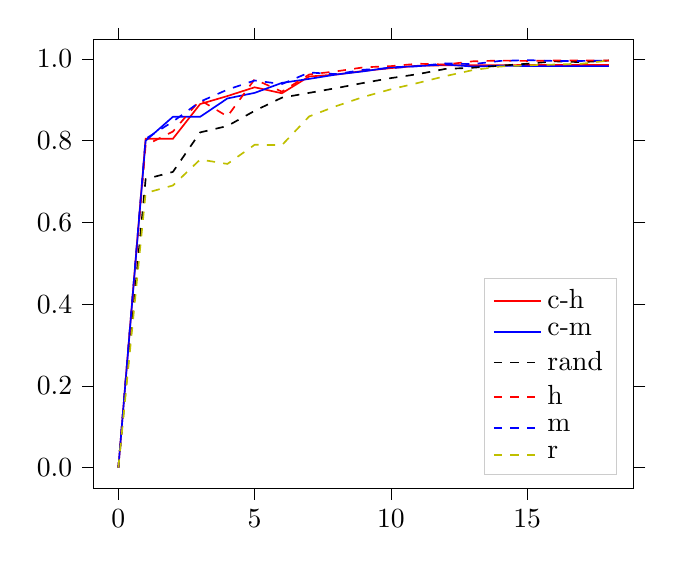
\begin{tikzpicture}

\definecolor{color0}{rgb}{0.75,0.75,0}

\begin{axis}[
legend cell align={left},
legend style={
  fill opacity=0.8,
  draw opacity=1,
  text opacity=1,
  at={(0.97,0.03)},
  anchor=south east,
  draw=white!80!black
},
tick align=outside,
tick pos=both,
x grid style={white!69.0196078431373!black},
xmin=-0.9, xmax=18.9,
xtick style={color=black},
y grid style={white!69.0196078431373!black},
ymin=-0.049853515625, ymax=1.046923828125,
ytick style={color=black},
ytick={-0.2,0,0.2,0.4,0.6,0.8,1,1.2},
yticklabels={−0.2,0.0,0.2,0.4,0.6,0.8,1.0,1.2}
]
\addplot [semithick, red]
table {%
0 0
1 0.8046875
2 0.8046875
3 0.8896484375
4 0.9091796875
5 0.9306640625
6 0.916015625
7 0.95703125
8 0.9619140625
9 0.970703125
10 0.9775390625
11 0.9833984375
12 0.984375
13 0.984375
14 0.984375
15 0.9853515625
16 0.9853515625
17 0.9853515625
18 0.9853515625
};
\addlegendentry{c-h}
\addplot [semithick, blue]
table {%
0 0
1 0.7998046875
2 0.8583984375
3 0.8583984375
4 0.9033203125
5 0.9169921875
6 0.94140625
7 0.951171875
8 0.9619140625
9 0.9697265625
10 0.9794921875
11 0.982421875
12 0.986328125
13 0.9814453125
14 0.9833984375
15 0.982421875
16 0.982421875
17 0.982421875
18 0.982421875
};
\addlegendentry{c-m}
\addplot [semithick, black, dashed]
table {%
0 0
1 0.7060546875
2 0.7236328125
3 0.8203125
4 0.8359375
5 0.873046875
6 0.9052734375
7 0.9169921875
8 0.9287109375
9 0.94140625
10 0.953125
11 0.962890625
12 0.9755859375
13 0.978515625
14 0.9833984375
15 0.98828125
16 0.994140625
17 0.9921875
18 0.99609375
};
\addlegendentry{rand}
\addplot [semithick, red, dashed]
table {%
0 0
1 0.7890625
2 0.822265625
3 0.8994140625
4 0.859375
5 0.9501953125
6 0.919921875
7 0.9619140625
8 0.9697265625
9 0.9794921875
10 0.982421875
11 0.98828125
12 0.986328125
13 0.994140625
14 0.99609375
15 0.9951171875
16 0.99609375
17 0.99609375
18 0.99609375
};
\addlegendentry{h}
\addplot [semithick, blue, dashed]
table {%
0 0
1 0.8046875
2 0.8466796875
3 0.8955078125
4 0.9248046875
5 0.947265625
6 0.9384765625
7 0.966796875
8 0.962890625
9 0.9736328125
10 0.9775390625
11 0.982421875
12 0.9892578125
13 0.9873046875
14 0.9951171875
15 0.9970703125
16 0.9951171875
17 0.9951171875
18 0.99609375
};
\addlegendentry{m}
\addplot [semithick, color0, dashed]
table {%
0 0
1 0.671875
2 0.6904296875
3 0.75390625
4 0.7431640625
5 0.7900390625
6 0.7890625
7 0.859375
8 0.884765625
9 0.9072265625
10 0.92578125
11 0.94140625
12 0.9580078125
13 0.97265625
14 0.9814453125
15 0.984375
16 0.986328125
17 0.98828125
18 0.99609375
};
\addlegendentry{r}
\end{axis}

\end{tikzpicture}

\hspace{0.9cm}
\caption{Aggregated cumulative costs and bounds.}
\label{fig:sx2}
\end{figure}

\begin{figure}[htp!]
\centering
% This file was created by tikzplotlib v0.9.8.
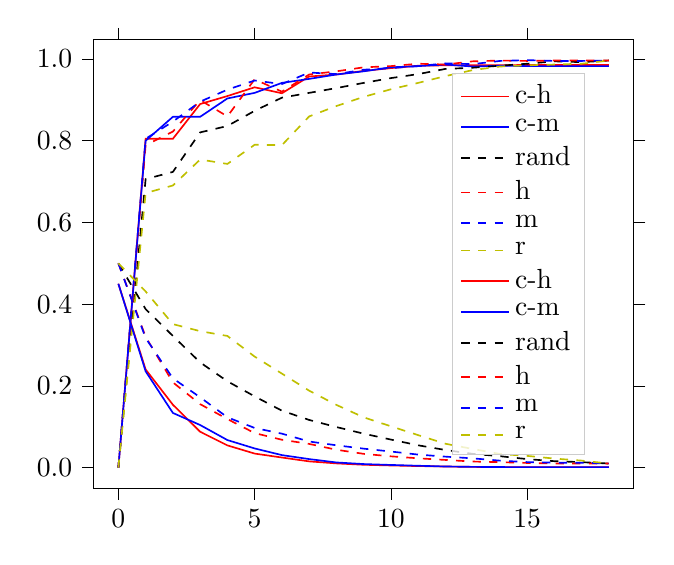
\begin{tikzpicture}

\definecolor{color0}{rgb}{0.75,0.75,0}

\begin{axis}[
legend cell align={left},
legend style={
  fill opacity=0.8,
  draw opacity=1,
  text opacity=1,
  at={(0.91,0.5)},
  anchor=east,
  draw=white!80!black
},
tick align=outside,
tick pos=both,
x grid style={white!69.0196078431373!black},
xmin=-0.9, xmax=18.9,
xtick style={color=black},
y grid style={white!69.0196078431373!black},
ymin=-0.049853515625, ymax=1.046923828125,
ytick style={color=black},
ytick={-0.2,0,0.2,0.4,0.6,0.8,1,1.2},
yticklabels={−0.2,0.0,0.2,0.4,0.6,0.8,1.0,1.2}
]
\addplot [semithick, red]
table {%
0 0
1 0.8046875
2 0.8046875
3 0.8896484375
4 0.9091796875
5 0.9306640625
6 0.916015625
7 0.95703125
8 0.9619140625
9 0.970703125
10 0.9775390625
11 0.9833984375
12 0.984375
13 0.984375
14 0.984375
15 0.9853515625
16 0.9853515625
17 0.9853515625
18 0.9853515625
};
\addlegendentry{c-h}
\addplot [semithick, blue]
table {%
0 0
1 0.7998046875
2 0.8583984375
3 0.8583984375
4 0.9033203125
5 0.9169921875
6 0.94140625
7 0.951171875
8 0.9619140625
9 0.9697265625
10 0.9794921875
11 0.982421875
12 0.986328125
13 0.9814453125
14 0.9833984375
15 0.982421875
16 0.982421875
17 0.982421875
18 0.982421875
};
\addlegendentry{c-m}
\addplot [semithick, black, dashed]
table {%
0 0
1 0.7060546875
2 0.7236328125
3 0.8203125
4 0.8359375
5 0.873046875
6 0.9052734375
7 0.9169921875
8 0.9287109375
9 0.94140625
10 0.953125
11 0.962890625
12 0.9755859375
13 0.978515625
14 0.9833984375
15 0.98828125
16 0.994140625
17 0.9921875
18 0.99609375
};
\addlegendentry{rand}
\addplot [semithick, red, dashed]
table {%
0 0
1 0.7890625
2 0.822265625
3 0.8994140625
4 0.859375
5 0.9501953125
6 0.919921875
7 0.9619140625
8 0.9697265625
9 0.9794921875
10 0.982421875
11 0.98828125
12 0.986328125
13 0.994140625
14 0.99609375
15 0.9951171875
16 0.99609375
17 0.99609375
18 0.99609375
};
\addlegendentry{h}
\addplot [semithick, blue, dashed]
table {%
0 0
1 0.8046875
2 0.8466796875
3 0.8955078125
4 0.9248046875
5 0.947265625
6 0.9384765625
7 0.966796875
8 0.962890625
9 0.9736328125
10 0.9775390625
11 0.982421875
12 0.9892578125
13 0.9873046875
14 0.9951171875
15 0.9970703125
16 0.9951171875
17 0.9951171875
18 0.99609375
};
\addlegendentry{m}
\addplot [semithick, color0, dashed]
table {%
0 0
1 0.671875
2 0.6904296875
3 0.75390625
4 0.7431640625
5 0.7900390625
6 0.7890625
7 0.859375
8 0.884765625
9 0.9072265625
10 0.92578125
11 0.94140625
12 0.9580078125
13 0.97265625
14 0.9814453125
15 0.984375
16 0.986328125
17 0.98828125
18 0.99609375
};
\addlegendentry{r}
\addplot [semithick, red]
table {%
0 0.449999999999992
1 0.240321093750003
2 0.154068750000002
3 0.0879601562499998
4 0.0545979492187504
5 0.0345669921874999
6 0.0248742187499998
7 0.0154591796875
8 0.0104958984375
9 0.00716503906250006
10 0.00544667968750006
11 0.00400634765625
12 0.00290869140625
13 0.00200585937499999
14 0.00137460937499999
15 0.00145478515624999
16 0.00144414062499999
17 0.00143984374999999
18 0.00143974609374999
};
\addlegendentry{c-h}
\addplot [semithick, blue]
table {%
0 0.449999999999992
1 0.235816308593751
2 0.133981542968751
3 0.1044369140625
4 0.0676275390624998
5 0.0471173828125
6 0.0308186523437499
7 0.0210914062499999
8 0.0128307617187499
9 0.00890488281249997
10 0.00674853515625
11 0.00476650390625
12 0.00295224609375002
13 0.00205888671875
14 0.00155673828125
15 0.00136240234375
16 0.00144453125
17 0.0014396484375
18 0.001439453125
};
\addlegendentry{c-m}
\addplot [semithick, black, dashed]
table {%
0 0.5
1 0.38800205078125
2 0.32236396484375
3 0.25762578125
4 0.21144267578125
5 0.1745076171875
6 0.139484375
7 0.116849609375
8 0.09946396484375
9 0.0832636718750001
10 0.0688158203125002
11 0.0547997070312502
12 0.0433041015625001
13 0.0339080078125
14 0.0281607421874999
15 0.0210115234374999
16 0.0159416015625
17 0.013575390625
18 0.0101943359375
};
\addlegendentry{rand}
\addplot [semithick, red, dashed]
table {%
0 0.5
1 0.3201904296875
2 0.20880224609375
3 0.155491015625001
4 0.118972656250001
5 0.0846564453125002
6 0.0683878906250001
7 0.0581800781250001
8 0.04395986328125
9 0.0338941406249999
10 0.0278213867187499
11 0.0230004882812499
12 0.01899560546875
13 0.0150919921875
14 0.0135923828125
15 0.0116212890625
16 0.01030810546875
17 0.0101529296875
18 0.0101943359375
};
\addlegendentry{h}
\addplot [semithick, blue, dashed]
table {%
0 0.5
1 0.317187499999997
2 0.218678808593748
3 0.172235253906248
4 0.123334277343749
5 0.0972216796875
6 0.0832712890624999
7 0.0641038085937499
8 0.0548044921874999
9 0.04663076171875
10 0.03955947265625
11 0.0320949218749999
12 0.0270456054687499
13 0.0228884765625
14 0.0172658203125
15 0.01367705078125
16 0.0123193359375
17 0.01206787109375
18 0.0101943359375
};
\addlegendentry{m}
\addplot [semithick, color0, dashed]
table {%
0 0.5
1 0.431250000000002
2 0.351269531249998
3 0.3340296875
4 0.322312109375
5 0.27181015625
6 0.23018603515625
7 0.188451464843749
8 0.15362529296875
9 0.123285546875
10 0.10120791015625
11 0.0796852539062503
12 0.0586057617187502
13 0.0458888671875001
14 0.0336228515625
15 0.02890341796875
16 0.022294140625
17 0.01733564453125
18 0.0101943359375
};
\addlegendentry{r}
\end{axis}

\end{tikzpicture}

\caption{Aggregated cumulative costs and bounds.}
\label{fig:sx}
\end{figure}

\subsection{Multi-Skill Experiments on Real Data}
For a validation on real data, we consider data xxx. Before the academic year begins, the students of the University of Applied Sciences and Arts of Southern Switzerland (SUPSI) are asked to take an online German language placement test with 95 questions. In years 2015 and 2016, the answers of 451 students to all the questions have been collected. 
	
\paragraph{Model elicitation.}
Four skills are assessed: \textit{W\"ortschatz} ($X_1$, vocabulary), 
\textit{Kommunikation} ($X_2$, communication), \textit{H\"oren} ($X_3$, listening), and \textit{Lesen} ($X_4$, reading). For each skill the student is assigned to a knowledge 
	level compliant with EU 
	guidelines.\footnote{\url{http://www.coe.int/t/dg4/linguistic/Source/Framework_EN.pdf}.}
	Levels A1, A2, B1, and B2 are considered, and skills are therefore modeled as 
	quaternary variables.
	Teachers associate each question with a single skill, which is set as the unique 
	background skill of the question. The number of questions associated with 
	$X_1$/$X_2$/$X_3$/$X_4$ is 26/24/30/15. The current evaluation method assigns 
	levels by setting thresholds on the percentage $\gamma$ of correct answers on each 
	skill (A1 if  $\gamma < 35\%$, A2 up to $55\%$, B1 up to $75\%$).\footnote{These data 
	as well as the software used for the simulations are freely available at 
	\url{http://ipg.idsia.ch/software.php?id=138}.}
	
	We first elicit from the teachers the structure of the BN/CN graph over the skills. The 
	result is a chain, which is augmented by leaf nodes modeling the questions, each 
	having its background skill as single parent. Overall, a tree-shaped topology as in 
	Fig.~\ref{fig:fourskills} is obtained. This makes exact inference in the BN fast, while in 
	the CN a variable elimination might be slow (a minute for query in our setup). A faster 
	approximate CN algorithm is therefore used \cite{antonucci2014e}.
	
	\begin{figure}[htp!]
		\centering
		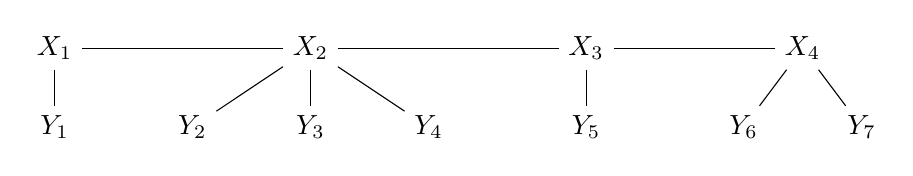
\begin{tikzpicture}%[scale=.8]
			\node[]  at (-0.25,0)  (w)  {$X_1$};
			\node[]  at (3,0) 		 (k)   {$X_2$};
			\node[]  at (6.5,0) 	(h)   {$X_3$};
			\node[]  at (9.25,0)   (l)    {$X_4$};
			\draw[] (w) -- (k);
			\draw[] (k) -- (h);
			\draw[] (h) -- (l);
			\node[]  at (-0.25,-1)(f1) {$Y_1$};
			\node[]  at (1.5,-1) 	 (f2) {$Y_2$};
			\node[]  at (3,-1) 	 (f3) {$Y_3$};
			\node[]  at (4.5,-1) 	(f4) {$Y_4$};
			\node[]  at (6.5,-1)	(f5) {$Y_5$};
			\node[]  at (8.5,-1)   (f6) {$Y_6$};
			\node[]  at (10,-1)  	(f7)  {$Y_7$};
			\draw[] (w) -- (f1);
			\draw[] (k) -- (f2);
			\draw[] (k) -- (f3);
			\draw[] (k) -- (f4);
			\draw[] (h) -- (f5);
			\draw[] (l) -- (f6);
			\draw[] (l) -- (f7);
		\end{tikzpicture}
		\caption{A directed graph for CAT\label{fig:fourskills}.}
	\end{figure}
	\vspace{-5mm}
	
	Teachers report their knowledge about the unconditional states of $X_1$ and the 
	conditional states of $X_i$ given $X_{i-1}$, for $i=2,3,4$, as qualitative judgments (top 
	of Tab.~\ref{tb:CPTs}). 
	To simplify the elicitation, the probabilities $P(X_i|X_{i-1})$ are given the same verbal 
	judgment for all $i=2,3,4$. A more detailed model could provide more accurate 
	evaluations but it would be very hard for the domain expert to elicit it in a reliable way. 
	Also, questions are divided by the teachers in three groups, corresponding to different 
	difficulty levels. Questions in the same group are quantified in the same way, 
	irrespective of their background skill, giving the judgments reported in the bottom part 
	of Tab.~\ref{tb:CPTs}. 
	
	{\small \begin{table*}[htp!] 
			\renewcommand{\arraystretch}{1.2}
			\centering
			{%\footnotesize
				\begin{tabular}{@{}lc@{}}
					\toprule
					$X_1$&$P(X_1)$\\
					\midrule
					A1&\emph{improbable}\\
					A2&\emph{uncertain}\\
					B1&\emph{uncertain}\\
					B2&\emph{improbable}\\
					\bottomrule
				\end{tabular}
				\quad
				\begin{tabular}{@{}lcccc@{}}
					\toprule	
					$P(X_i|X_{i-1})$&\phantom{.}$X_{i-1}=\mathrm{A1}$\phantom{.}&\phantom{.}$X_{i-1}=\mathrm{A2}$\phantom{.}&\phantom{.}$X_{i-1}=\mathrm{B1}$\phantom{.}&\phantom{.}$X_{i-1}=\mathrm{B2}$\phantom{.}\\
					\midrule
					$X_i$=A1&\emph{fifty-fifty}&\emph{uncertain}&\emph{improbable}&\emph{impossible}\\
					$X_i$=A2&\emph{uncertain}&\emph{fifty-fifty}&\emph{uncertain}&\emph{improbable}\\
					$X_i$=B1&\emph{improbable}&\emph{uncertain}&\emph{fifty-fifty}&\emph{uncertain}\\
					$X_i$=B2&\emph{impossible}&\emph{improbable}&\emph{uncertain}&\emph{fifty-fifty}\\
					\bottomrule
			\end{tabular}}
			\vskip 2mm
			\begin{tabular}{@{}lcccc@{}}\toprule
				$P(Y=T|X)$\phantom{aa}&\phantom{a}$X=\mathrm{A1}$\phantom{a}&\phantom{a}$X=\mathrm{A2}$\phantom{a}&\phantom{a}$X=\mathrm{B1}$\phantom{a}&\phantom{a}$X=\mathrm{B2}$\phantom{a}\\
				\midrule
				Easy&\emph{uncertain}&\emph{fifty-fifty}&\emph{expected}&\emph{probable}\\
				Medium&\emph{improbable}&\emph{uncertain}&\emph{fifty-fifty}& 
				\emph{expected}\\
				Difficult&\emph{impossible}&\emph{improbable}&\emph{uncertain}& 
				\emph{fifty-fifty}\\
				\bottomrule
			\end{tabular}
			\vskip 2mm
			\caption{Expert judgements.}\label{tb:CPTs}
	\end{table*}}
	%\vspace{-10mm}
	For the CN, those judgements are translated in interval constraints for the 
	corresponding events on the basis of the verbal-numerical scale in Tab.~\ref{tb:labels}. 
	Different probability intervals are considered for skills and questions as they refer to 
	events of different type. For instance, when the expert considers ``\emph{impossible}'' 
	for an A1 level student to know the answer to a difficult question, the student is 
	assigned a probability between .175 and .2 of answering correctly, as the questions 
	offer only four choices plus the option of giving no answer. 
	Notice that, by doing so, we are not anymore assuming that all questions in the same 
	difficulty group share exactly the same conditional PMFs (as done by the BN model), as 
	PMFs of different questions can vary independently in the given intervals. This seems a 
	more sensible assumption than that of the precise model.
	For the BN, the PMFs corresponding to the centers of mass of the CSs defining the CN 
	are used. Numerical inferences in the BN are consequently included in the intervals 
	computed with the CN.
	
	{\small
		\begin{table*}[htp!] 
			\renewcommand{\arraystretch}{1.2}
			\centering
			\begin{tabular}{@{}lcccccc@{}}
				\toprule
				Judgement&\emph{impossible}&\emph{improbable}&\emph{uncertain}&\emph{fifty-fifty}&\emph{expected}&\emph{probable}\\
				\midrule
				Skills&$1$-$10\%$&$10$-$20\%$&$20$-$40\%$&$30$-$50\%$&-&-\\
				Questions&$17.5$-$20\%$&$22.5$-$25\%$&$30$-$35\%$&$60$-$65\%$&$75$-$80\%$&
				 $95$-$97.5\%$\\
				\bottomrule
			\end{tabular}
			\caption{A verbal-numerical scale for probability-intervals 
			elicitation.}\label{tb:labels}
	\end{table*}}
	
	\paragraph{Experimental results.} 
	%Acronyms BN-NA, CN-NA, BN-AD, CN-AD denote 
	BN and CN methods in their non-adaptive (NA) and adaptive (AD) versions are 
	considered. \emph{Accuracy}, i.e., the proportion of students to whom the test assigns 
	the same level of the current evaluation method, describes BN performances. This 
	measure cannot be used for the set-valued outputs of CN methods. In this case the 
	$u_{65}$ measure can provide a comparison with the accuracy 
	\cite{zaffalon2012evaluating}. If $\mathcal{L}$ is the set of levels assigned by the CN 
	on a skill and $L$ its cardinality, a \emph{discounted} accuracy gives $1/L$ if 
	$\mathcal{L}$ includes the true level and zero otherwise. The $u_{65}$ is a concave 
	reinforcement of this score based on risk-adverse arguments. Its underlying 
	assumption is that acknowledging the indecision between more levels has larger utility 
	than randomly choosing one of them (e.g., the teacher could set up further 
	assessments in the undecided cases). Tab.~\ref{tb:nonAdaptiveResults} shows the NA 
	comparison. In Fig.~\ref{fig:plots} (left), the BN-NA accuracy is separately evaluated on 
	the determinate (light bars) and indeterminate (dark bars) instances, i.e. those for 
	which, respectively, a single level or multiple levels are returned by the CN model. On 
	average, CN-NA returns single levels in $37.25\%$ of the cases and, if this is not the 
	case, an average of $2.36$ levels ($3.22$ with interval dominance) are returned. 
	
	\begin{table*}[htp!]
		\centering
		\begin{tabular}{@{}lccccc@{}}\toprule
			Algorithm&\phantom{aa}Average\phantom{aa}&\phantom{aaa}$X_1$\phantom{aaa}&\phantom{aaa}$X_2$\phantom{aaa}&
			 \phantom{aaa}$X_3$\phantom{aaa}&\phantom{aaa}$X_4$\phantom{aaa}\\
			\midrule
			BN-NA (acc)&$63.09\%$&$	67.56	\%$&$60.85\%$&${	75.84	
			\%}$&$48.10\%$\\
			CN-NA ($u_{65}$)& ${65.37\%}$&$67.71\%$&${66.67\%}$&$	
			70.33\%$&${56.76\%}$\\
			\bottomrule
		\end{tabular}
		\caption{Non-adaptive tests results.}\label{tb:nonAdaptiveResults}
	\end{table*}
	
	In the AD case we also track the average number of asked questions. Results are in 
	Fig.~\ref{fig:plots} (right). CN-AD (circles) is tested for different thresholds over the 
	entropy (labels of the markers) against a version of BN-AD based on the joint entropy 
	(triangles). Similar values are obtained by coping with marginal entropies. We also allow 
	the BN-AD method to return multiple levels by maximizing the expected $u_{65}$ utility 
	over any possible set of levels. This variant is called BN-AD' and the corresponding 
	$u_{65}$ measure is reported  (squares).
	
	\begin{figure}[htp!]
		\centering
		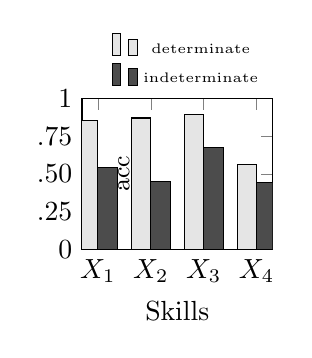
\begin{tikzpicture}
			\begin{axis}[width=4cm,height=3.5cm,ybar=0,bar width=7pt,ylabel={\small acc}, 
			xlabel={Skills},xtick=data,ytick={0,25,50,75,100},ymin=0,ymax=100,yticklabels={0,.25,.50,.75,1},symbolic
			 x coords={$X_1$,$X_2$,$X_3$,$X_4$}, y label style={at={(axis description 
			cs:0.3,.5)},anchor=south},xtick align=inside, legend 
			style={at={(1,1)},anchor=south east},legend style={draw=none}]
				\addplot[fill=black!10] coordinates 
				{($X_1$,85.42)($X_2$,87.06)($X_3$,89.51)($X_4$,56.34)}; 
				\addlegendentry{\tiny{determinate}} 
				\addplot[fill=black!70] coordinates 
				{($X_1$,54.51)($X_2$,45.13)($X_3$,67.72)($X_4$,44.26)};
				\addlegendentry{\tiny{indeterminate}}
			\end{axis}
		\end{tikzpicture}
		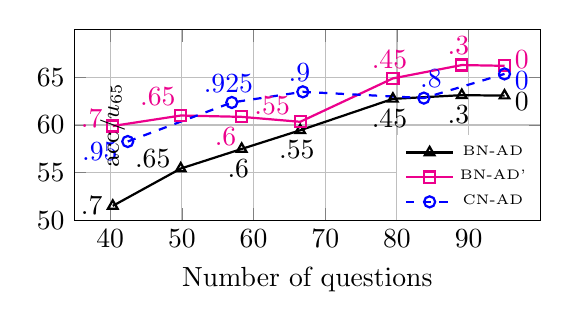
\begin{tikzpicture}
			\begin{axis}[width=7.5cm,height=4cm,ylabel={\small 
			acc/$u_{65}$},xlabel={Number of questions},xmin=35, xmax=100,ymin=50, 
			ymax=70, xtick={40,50,60,70,80,90}, ytick={50,55,60,65},legend 
			style={at={(1,0)},anchor=south east},ymajorgrids=true,xmajorgrids=true,  y label 
			style={at={(axis description cs:0.13,.5)},anchor=south},legend style={draw=none}]
				\addplot[black,thick,mark=triangle,mark options={fill=black}, visualization 
				depends on=\thisrow{alignment} \as \alignment, nodes near coords, point 
				meta=explicit symbolic,  every node near coord/.style={anchor=\alignment}] 
				table [meta index=2 ] {
					x y label alignment
					40.36	51.51 .7 0
					49.84	55.43 .65 -20
					58.34	57.49 .6 80
					66.50 59.45 .55 80
					79.43	62.75 .45 80
					89.04	63.14 .3 80
					95  63.09     0  160
				};
				\addlegendentry{\tiny{BN-AD}}
				\addplot[magenta,thick,mark=square,mark options={fill=black}, visualization 
				depends on=\thisrow{alignment} \as \alignment, nodes near coords, point 
				meta=explicit symbolic,  every node near coord/.style={anchor=\alignment}] 
				table [meta index=2 ] {
					x y label alignment
					40.36	59.9 .7 -20
					49.84	61.00 .65 -40
					58.34	60.86 .6 50
					66.50 60.34 .55 -30
					79.43	64.90 .45 -80
					89.04	66.3 .3 -80
					95  66.22     0  -160
				};
				\addlegendentry{\tiny{BN-AD'}}
				\addplot[dashed,blue,thick,mark=o,mark options={solid,fill=white},
				visualization depends on=\thisrow{alignment} \as \alignment,
				nodes near coords, % Place nodes near each coordinate
				point meta=explicit symbolic, % The meta data used in the nodes is not 
				%explicitly provided and not numeric
				every node near coord/.style={anchor=\alignment} ] table [meta index=2 ] {
					x       y   label  alignment
					42.45 58.27  .95   20
					56.96 62.37  .925   -80
					66.87 63.49   .9   -80
					83.75 62.83  .8    -110
					95   65.37   0  160
				};
				\addlegendentry{\tiny{CN-AD}}
			\end{axis}
		\end{tikzpicture}
		\caption{Non-adaptive (left) and adaptive (right) tests performance.}\label{fig:plots}
	\end{figure}
	
	
	As a comment, CNs seem to identify hard-to-evaluate students as those for which 
	multiple levels are provided. In fact, the agreement between the BN and the traditional 
	tests is larger when the CN test is determinate. As a consequence, the CN $u_{65}$ 
	measure is, on average, larger than the BN accuracy. 
	A limitation of the CN test is the large fraction of indeterminate evaluations. One can 
	interpret this result as a lack of robustness of the BN model, as even small variations in 
	the model specifications can result in different decisions. Results also show that, both 
	BN-AD and CN-AD approaches reduce the number of questions asked without 
	significantly affecting the accuracy. BN-AD performances are improved by the ``credal'' 
	variant BN-AD'. The results becomes very similar to those of the CN-AD. Yet, the latter 
	method appears to be a more principled and suitable approach for a direct modeling of 
	qualitative expert knowledge. 
	
	%does not require any, potentially questionable, imputation of the probabilistic ranges 
	%provided by the experts.
	
	%Yet, we regard theof BN-AD, we regard the CN approach as more principled and 
	%suitable for a direct modeling of qualitative expert knowledge.
	
	%uch a difference disappear if the credal-like variant BN-AD' is considered.
	%However, the CN-AD procedure appears to be more effective, as the $u_{65}$ 
	%accuracy measure decreases more slowly than the accuracies of BN-AD procedures.  
	%Finally,comparing the two BN-AD approaches, one can see that the use of the local 
	%instead of the joint entropy does not compromise the effectiveness of the adaptive 
	%approach. 
	
	
\section{Outlooks and Conclusions}\label{sec:conc}
A new approach to the xxx.


%\footnote{Extension to non Boolean answers is trivial as all answers $Y_i$ are \emph{manifest} variables, and, thus, $Y_i$ can be always regarded as a binary variable with the two values denoting the observed answer $y_i$ and its negation \cite{antonucci2009}.} 
%We call \emph{background} of a question the set of skills ``required'' to answer it. This can be regarded as a conditional independence statement: given the background skills, the answer to the question is independent of the other skills and of the other questions. 

%\paragraph{Expert knowledge modeling.} For a reliable expert knowledge modeling, we use CSs induced by \emph{probability intervals}. Qualitative judgments about the probability of a state are converted in interval constraints such as $l\leq P(x) \leq u$, with the interval $[l,u]$ capturing the expert knowledge behind the judgment in a more reliable way than a sharp assessment. The CS consistent with these constraints is eventually obtained by standard polyhedral algorithms. Verbal to interval-numeric scales such as that Tab.~\ref{tb:labels} are used. For instance, if for the probability of the true state of the Boolean variable $Y$ the expert judgment is ``very likely'', the 	corresponding linear constraint is $.2 \leq P(Y=\textrm{true}) \leq .4$.

%The task displays higher complexity than in the case of BNs (e.g., exact inference in non-binary singly-connected CNs is NP-hard \cite{maua14jair}), but approximate techniques can be considered when exact inference is unfeasible \cite{antonucci2014e}. 
	
%To compare the posterior intervals and decide the actual level of the student we might adopt the (conservative) \emph{interval dominance} criterion \cite{troffaes}, which rejects a level if its upper probability is smaller than the lower probability of some other level. Overlaps between intervals might therefore induce a situation of \emph{indecision} between two or more levels. This is a so-called \emph{credal} classification of the student level \cite{zaffalon2012evaluating}, and it represents the fact that students answers are somehow contradictory or not informative enough to provide a sharp decision. 
	
%This topic has been the subject of much discussion \cite{klir1999uncertainty}. A cautious approach \cite{abellan2003maximum} consists in taking the upper entropy $\overline{H}(\bm{X})$, i.e., the entropy of the most entropic PMF in the convex closure $\overline{K}(\bm{X})$ of  $K(\bm{X})$. In our framework, we should, then, look for maximum values of conditional entropies, such as $\overline{H}(X_i|Y',\bm{y})$ or $\overline{H}(X_i|\Pi_{X_i})$, as conditional  entropies are required to compute both: (i) the joint (unconditional) entropy $H(\bm{X})$ (and its posterior values); and (ii) the conditional entropies  involved in the  question selection in Eq.~\eqref{eq:expent}.By definition a conditional entropy is a convex combination (whose weights are the elements of a marginal PMF) of convex functions (the entropies). The objective function might, then, be non-convex, as the weights are also optimization variables.

	
		Comment 4: The optimisation in the credal setting shouldn't be the following one?
	
	$$\max_P [\max_s P(s,q=0)+\max_s P(s,q=1)]$$ 
	
	$\P(s,q=0)$ and $P(s,q=1)$ are both functions of $p, \pi_0,$ and $\pi_1$ so I do not 
	think we can split the optimization
	
	$$\max_P \max_s P(s,q=0)+\max_P\max_s P(s,q=1)$$ 
	
	However, it could be a reasonable approximation. Then, we can switch the optimization 
	over $P$ and $s$ because they are both max, and obtain: 
	$$\max_s \overline{P}(s)\overline{P}(q=0|s)+\max_s  \overline{P}(s)\overline{P}(q=1|s)$$.
	
	If instead we are looking for the minimum over P, we cannot switch the optimization 
	over $P$ and $s$:
	$$\min_P \max_s P(s,q) \neq \max_s \min_P P(s,q)$$.
	
	However I think we can split the optimization into 4 quadratic optimizations.
	Let's use the following parametrization:
%	\begin{multline}\label{eq:minimization}
%		\min_{p,\pi_0,\pi_1} \sigma_Q(p,\pi_0,\pi_1) = \\
%		2\min_{p,\pi_0,\pi_1} \bigl( \max\{\pi_1 p, \pi_0 (1-p)\} + \\
%		~~~ \max\{(1-\pi_1 )p, (1-\pi_0) (1-p)\} \bigr) \approx \\
%		2 \bigl( \min_{p,\pi_0,\pi_1}  \max\{\pi_1 p, \pi_0 (1-p)\} + \\
%		~~~ \min_{p,\pi_0,\pi_1} \max\{(1-\pi_1 )p, (1-\pi_0) (1-p)\} \bigr) 
%	\end{multline}
	
	Let's consider the first optimization $\min_{p,\pi_0,\pi_1}  \max\{\pi_1 p, \pi_0 (1-p)\}$. It 
	can be written as
	$$ \min(\tilde{P}(s=0,q),\tilde{P}(s=1,q)) $$ 
	where 

%	\begin{multline}
%		\tilde{P}(s=0,q) = \min_{\pi_1 ,p} \pi_1 p \\
%		\begin{array}{ll}
%			\text{subject to} & \pi_1 p > \pi_0 (1-p) \\
%			~&\underline{x} \leq x\leq \overline{x}\\ 
%		\end{array}
%	\end{multline}
	and 
%	\begin{multline}
%		\tilde{P}(s=1,q) = \min_{\pi_0 ,p} \pi_0 (1-p) \\
%		\begin{array}{ll}
%			\text{subject to} & \pi_1 p < \pi_0 (1-p)\\
%			~&\underline{x} \leq x\leq \overline{x}\\ 
%		\end{array}
%	\end{multline}
	
	where the constraint $x = (\pi_0, \pi_1 ,p)$.
	
	In general, let $N_s$ be the number of skill levels and $N_q$ the number of possible 
	answers, then the number of quadratic optimizations to solve should be equal to 
	$N_s\cdot N_q$. 
	
	In this two dimensional example, we might not need the approximation above as the 
	minimization in \ref{eq:minimization} can be written as $\min_{i=1:4}(\tilde{P}_1)$, where
	
%	\begin{multline}
%		\tilde{P}_1 = \min_{\pi_0,\pi_1,p} \pi_1 p+ (1-\pi_1)p = p \\
%		\begin{array}{ll}
%			\text{subject to} & \pi_1 p > \pi_0 (1-p) \\
%			~&  (1-\pi_1)p > (1-\pi_0)(1-p)  \\
%			~&\underline{x} \leq x\leq \overline{x}\\ 
%		\end{array}
%	\end{multline}
	and so on. However, in this case, the number of optimizations to solve should be 
	$N_s^{N_q}$, that is, it grows exponentially with  $N_q$. 
	
	Then, to bypass this non-convex optimization task, we compute (i) by separately considering the entropies of each skill $X_i\in\bm{X}$. This is analogous to the marginal approach commonly considered in multi-label classification to minimize Hamming losses 
	\cite{antonucci2016c}. The issue (ii) is more challenging. We consider the following 
	upper approximation of $\overline{H}(X_i|Y',\bm{y})$:
	\begin{equation}
		\overline{\overline{H}}(X_i|Y',\bm{y})=
		\max_{P(y'|\bm{y})\in
			\{\underline{P}(y'|\bm{y}),\overline{P}(y'|\bm{y})\}}
		\sum_{y' \in \{\textrm{true},\textrm{false}\}}
		\overline{H}(X_i|\bm{y},y') P(y'|\bm{y})\,,
	\end{equation}
	where the bounds of $P(y'|\bm{y})$ are obtained by standard CN updating algorithms.
	The problem thus reduces to the computation of upper entropies as
	\begin{equation}\label{eq:entropy}
		\overline{H}(X_i|\bm{y}) := \sup_{P(X_i|\bm{y}) \in \overline{K}(X_i|\bm{y})} 
		H(X_i|\bm{y})\,,
	\end{equation}
	where  $\overline{K}(X_i|\bm{y})$ is the posterior CS after conditioning on the observed 
	answers $\bm{y}$.  If $\overline{K}(X_i|\bm{y})$ has a finite number of non-inner 
	points, this is a linearly-constrained convex optimization whose solution typically 
	corresponds to either the uniform PMF or a non-inner point on the frontier of 
	$\overline{K}(X_i|\bm{y})$. A numerical solution can be easily found by a simple iterative 
	approach in the special case of CS specified by probability intervals 
	\cite{abellan2003maximum}. We have therefore computed the posterior lower and 
	upper bounds of $P(X_i|\bm{y})$, and then maximized the entropy with respect to 
	those bounds. % as in Eq.~\eqref{eq:entropy}. 
	The procedure induces an outer approximation of $\overline{K}(X_i|\bm{y})$, and hence 
	the upper approximation  of the maximum entropy 
	$\overline{\overline{H}}(X|\bm{y})\geq\overline{H}(X|\bm{y})$. 
	%With a small notation abuse such approximate value is also denoted as 
	%$\overline{H}(X|\bm{y})$ and is regarded here as a measure of the informativeness 
	%level 
	%achieved for skill $X$ after the answers $\bm{y}$. 
	Finally, to generalise Eq.~\ref{eq:strongext} to CNs, we define the information gain 
	provided by a question $Y'$ for its background skill $X_{Y'}$ as 
	$\overline{\overline{H}}(X_{Y'}|\bm{y})-\overline{\overline{H}}(X_{Y'}|Y',\bm{y})$ and 
	select the question $\tilde{Y}'$ leading to the maximum information gain, i.e.,
	\begin{equation}\label{eq:credalentropy}
		\tilde{Y}' := \arg \max_{Y'\in\bm{Y}'} 
		\bigl[
		\overline{\overline{H}}(X_{Y'}|\bm{y})-\overline{\overline{H}}(X_{Y'}|Y',\bm{y}) 
		\bigr]
		\,.
	\end{equation}
	For the stopping criterion, as we do not consider the joint entropy over the skills, we 
	separately require each $\overline{\overline{H}}(X_i|\bm{y})$ to be smaller than a 
	threshold $\tilde{H}$. To be consistent with this choice, we remove from the set of 
	questions to be selected, those whose background skills already satisfy this condition.
	
	Note that the use of an outer approximation of the upper entropy affects only the 
	question selection process (eventually making it sub-optimal), whereas it has no effect 
	on the student evaluation given a set of answers.
	
	

		\begin{theorem}
		\begin{equation}
			\max_{x}  \max \{ f(x) , g(x) \}  
			=
			\max \{ \max_{x'} f(x') , \max_{x''} g(x'') \} 
		\end{equation}
		Let 
		$$y^{*}:=\max_x \max\{f(x),g(x)\}$$
		$$y^{**}:= \max \{ \max_{x'} f(x') , \max_{x''} g(x'') \}$$
		Say for instance that $y^{**}=max_x f(x)$ and let $x^{**}:=\arg\max_x f(x)$. Thus:
		$$f(x^{**})\geq \max_{x'} g(x) \geq g(x^{**})$$ 
		
		Let $x^{*}:= \arg\max_x \max\{f(x),g(x)\}$. 
		It cannot be $y^{*}:=g(x^{*})$ as this would imply $g(x^{*}) \geq f(x^{*})$ 
		
		
		%Assume ad absurdum $y^{*}\neq y^{**}$.
		
		
		If $y^{*}:=f(x^{*})$ we should have $y^{*}=y^{**}$.
		Vice versa, 
		
		or
		%$y^{*}:=g(x^{*})$. In the first case 
	\end{theorem}
	

\bibliographystyle{splncs04}
\bibliography{biblio}
\end{document}

\subsection*{Toy Example}
	Consider a Boolean skill $S$ with states $s_0$ and $s_1$ and a Boolean 
	question/answer $Q$. Let us shape the model as a BN, $S\to Q$. The prior $P(S)$ is 
	specified by a parameter $p:=P(s_1)$. The question CPT $P(Q|S)$ might be specified 
	instead by two parameters $\pi_1:=P(q_1|s_1)$ and $\pi_0:=P(q_1|s_0)$. The 
	informativeness score we assign two the question is
	\begin{equation}
		\sigma_Q = H[S|Q]:=H[S|q_0]P(q_0)+H[S|q_1]P(q_1)\,.
	\end{equation}
	We have
	\begin{equation}
		P(q_1)=\pi_1 p + \pi_0 (1-p)
	\end{equation}
	while $P(q_0)=1-P(q_1)$ and also
	\begin{equation}
		P(s_1|q_1)=\frac{\pi_1 p}{\pi_1 p + \pi_0 (1-p)}=\frac{1}{1+\frac{\pi_0(1-p)}{\pi_1 p}}
	\end{equation}
	and
	\begin{equation}
		P(s_1|q_0)=\frac{p (1-\pi_1)}{p(1-\pi_1) +  (1-p)(1-\pi_0)} = \frac{1}{1+ \frac{ 
		(1-p)(1-\pi_0)}{p (1-\pi_1)}} 
	\end{equation}
	while $P(S=0|Q=1)$ by normalization. Accordingly:
%	\begin{multline}
%		\sigma_Q(p,\pi_0,\pi_1)=\\
%		h \circ f[\gamma/l(p)] \cdot t +
%		h \circ f[\gamma'/l(p)] \cdot (1-t)\,
%		%\theta(\frac{\pi_0(1-p)}{\pi_1 p}) [\pi_1 p + \pi_0 (1-p)]\\
%		%+ \theta(\frac{ (1-p)(1-\pi_0)}{p (1-\pi_1)}) [1-\pi_1 p + \pi_0 (1-p)]
%	\end{multline}
	where $\gamma = \frac{\pi_0}{\pi_1}$, $\gamma' = \frac{1-\pi_0}{1-\pi_1}$, and $t = \pi_1 
	p + \pi_0 (1-p)$.
	
	{\color{blue}{In other words:
			$\sigma_Q(p,\pi_0,\pi_1):= G(\frac{1-p}{p} \frac{1-\pi_0}{1-\pi_1}) (1-p) + 
			G(\frac{1-p}{p} \frac{\pi_0}{\pi_1}) p$}}
	
	
	
	An alternative score might be achieved by replacing $h$ with $m$, i.e.,
	\begin{equation}
		\sigma_Q' := 
		m \circ f[\gamma/l(p)] \cdot t +
		m \circ f[\gamma'/l(p)] \cdot (1-t)\,
	\end{equation}
	As $f$ is monotone, we can commute $m$ and $f$ *** explain ***, i.e.,
	\begin{equation}
		\sigma_Q' := 
		f \circ m[\gamma/l(p)] \cdot t +
		f \circ m[\gamma'/l(p)] \cdot (1-t)\,
	\end{equation}
	with, as $\gamma>0$. $f \circ m[\gamma/l(p)] = f[\gamma m(l(p))]$
	We can similarly define another score $\sigma_Q''$ based on $\tilde{i}_\epsilon$.
	\subsection*{Explicit maximization}
	$$H[S|Q]\simeq \sigma_Q' = \sum_q P(s^*(q)|q) P(q)$$
	where $s^*(q):=\arg\max_s P(s|q)$. 
	$$\sigma_Q'= \sum_q P(s^*(q),q) = \sum_q P(s^*(q) P(q|s^*(q))$$
	Note that, if $s^*(q)$ is the same for each $q$, the score just corresponds to $P(s^*)$. 
	In other words, the score is flat is each answer gives the same most likely skill level *** 
	reasonable ***. Let us move to an imprecise setting and intend the $s^*$ state as
	$s^*(q):=\arg\max_s \overline{P}(s|q)$. The objective function is a linear combination of 
	$P(s*(q)$ whose coefficient can be optimized independently. Overall, this corresponds 
	to a linear programming task.
	$$\max_s \overline{P}(s,q) = \max_s \max_P P(s) P(q|s) = \max_s \overline{P}(s) 
	\overline{P}(q|s)$$
	
	\subsection*{Francesca's comments}
	
	Comment1: This sentence is not clear to me:  "as $\gamma>0$. $f \circ m[\gamma/l(p)] 
	= f[\gamma m(l(p))]$".\\
	Comment2: How shall we use the Gumbel's trick
	
	
	Comment 3: Below I obtain something that looks different to me, but maybe it is 
	equivalent.  
	
	\begin{equation}
		P(s_1|q_1)=\frac{\pi_1 p}{P(q_1)}
	\end{equation}
	
%	\begin{multline}
%		\sigma_Q(p,\pi_0,\pi_1)=\\
%		m\bigl(\frac{\pi_1 p}{P(q_1)}\bigr) \cdot P(q_1)  +
%		m\bigl(\frac{(1-\pi_1) p}{1-P(q_1)}\bigr) \cdot (1-P(q_1))\,
%	\end{multline}
	
	But, as $P(q_1)\geq 0$, then
%	\begin{multline}
%		m\bigl(\frac{\pi_1 p}{P(q_1)}\bigr) =\\
%		2max\bigl(\frac{\pi_1 p}{P(q_1)},1-\frac{\pi_1 p}{P(q_1)} \bigr) =\\
%		2max\bigl(\frac{\pi_1 p}{P(q_1)},\frac{\pi_0(1- p)}{P(q_1)} \bigr) =\\
%		\frac{2}{P(q_1)}max\bigl(\pi_1 p,\pi_0(1- p)\bigr).\\
%	\end{multline}
	
	Similarly, as $1-P(q_1)\geq 0$, 
%	\begin{multline}
%		m\bigl(\frac{(1-\pi_1) p}{1-P(q_1)}\bigr) =\\
%		\frac{2}{1-P(q_1)}max\bigl((1-\pi_1) p,(1-\pi_0)(1- p)\bigr),\\
%	\end{multline}
	
	so that,
	
%	\begin{multline}
%		\sigma_Q(p,\pi_0,\pi_1)= \\
%		2 max\{\pi_1 p, \pi_0 (1-p)\}+
%		2 max\{(1-\pi_1 )p, (1-\pi_0) (1-p)\}\,
%	\end{multline}
	
	\subsection*{Formulae}
	Let us define the functions, all defined for $x\in [0,1]$, apart from $f$ defines for each 
	$x\geq 0$:
	\begin{eqnarray}
		f(x)&:=& \frac{1}{1+x},\,,\\
		h(x)&:=&-x \cdot \log_2 x - (1-x)  \cdot \log_2 (1-x)\,,\\
		l(x)&:=&\frac{x}{1-x}\,,\\
		m(x)&:=&2 \max\{x,1-x\}\,,\\
		i_\epsilon(x)&:=&\epsilon\log(e^{\frac{2x}{\epsilon}}+e^{\frac{2(1-x)}{\epsilon}})\,,\\
		\tilde{i}_\epsilon(x)&:=&\frac{i_\epsilon(x)-i_\epsilon(0)}{i_\epsilon(\frac{1}{2})-i_\epsilon(0)}\,.
	\end{eqnarray}
	
	Derivatives:
	\begin{eqnarray}
		f'(x)&:=& -\frac{1}{(1+x)^2},\,,\\
		h'(x)&:=&\log_2 \frac{1-x}{x}\,\\
		G(x) &:=& h \circ f(x)\,\\
		G'(x) &:=& h[f(x)] f'(x)=-\frac{\log_2\frac{1-f(x)}{f(x)}}{(1+x)^2}\,\\
		G'(x) &:=& -\frac{\log_2 x}{(1+x)^2}\,\\
		l(x)&:=&\frac{x}{1-x}\,,\\
		m(x)&:=&2 \max\{x,1-x\}\,,\\
		i_\epsilon(x)&:=&\epsilon\log(e^{\frac{2x}{\epsilon}}+e^{\frac{2(1-x)}{\epsilon}})\,,\\
		\tilde{i}_\epsilon(x)&:=&\frac{i_\epsilon(x)-i_\epsilon(0)}{i_\epsilon(\frac{1}{2})-i_\epsilon(0)}\,.
	\end{eqnarray}
	
	
A few remarks. Function $f$ is a monotonically decreasing function with values in 
$[0,1]$. Function $h(x)$ corresponds to the entropy of a mass function over a Boolean 
	variable with a probability equal to $x$. On the extreme points of its domain, we take 
	the limit value, i.e., zero. The function is unimodal and achieve its maximum on  
	$x=\frac{1}{2}$. Function $l$ is the popular \emph{logit} function, it is monotonically 
	increasing function of $x$ and $l(1-x)=l(x)^-1$. Function $m(x)$ is $x$ for $x\geq 
	\frac{1}{2}$ and $1-x$ otherwise. 
	Exactly as $h$, functions $m$ and $\tilde{i}_\epsilon$, for each $\epsilon>0$, have the 
	same (zero) value for $x=0$ and $x=1$, being all unimodal with maximum in 
	$x=\frac{1}{2}$.
	Finally, the popular Gumbel's trick implies:
	\begin{equation}
		\lim_{\epsilon \to 0} i_\epsilon(x)= 
		\lim_{\epsilon \to 0} \tilde{i}_\epsilon(x)
		= m(x)\,.
	\end{equation}